\documentclass[11pt]{article}
\usepackage[top=1in, bottom=1in, left=1in, right=1in]{geometry}
\usepackage{amssymb}
\usepackage{physics}

\usepackage{listings}
\lstset{frame = tb, language = Python,
		aboveskip = 3mm, belowskip = 3mm,
		tabsize = 3, columns = flexible,
		basicstyle = \small\ttfamily}

\usepackage{graphicx}
\graphicspath{{c:/Users/Jacob/Documents/Coding_Stuff/LaTeX/Honors_Thesis/Figures/}}

\usepackage{fancyhdr}
\pagestyle{fancy}
\renewcommand{\sectionmark}[1]{\markboth{#1}{}}
\fancyhf{}
\fancyhead[R]{\leftmark}
\fancyhead[L]{Monte Carlo and Lattice QCD}
\fancyfoot[C]{\thepage}
\fancypagestyle{plain}{\fancyhf{}
	\renewcommand{\headrulewidth}{0pt}}

\usepackage{tikz}
\usetikzlibrary{shapes.callouts}
\tikzset
{
	line/.style = {black},
	transition/.style = {dashed, black}
}

\begin{document}

\section{Lattice Quantum Chromodynamics}
We now shift our focus to quantum chromodynamics (QCD). The field of QCD is the study of the strong interaction, one of the four fundamental forces, that describes the interactions between quarks and gluons, the mediator of the strong force. And together quarks and gluons make up hadrons (e.g. protons). Lattice QCD is a nonperturbative approach for modeling and calculating QCD measurements\footnote{The importance of lattice QCD being nonperturbative is described in the introduction but is due to the large coupling constant of the strong force.}. On the lattice, the quarks live on the sites while the gluon fields exists on the links.

In some ways it is analogous to the previous section in that instead of space coordinates $x(t)$, we deal with fields dependent on $x=(\vb{x},t)$ where $x$ is now a spacetime point. The lattice is now four dimensional and thus size of the lattice $N$ will have a much greater effect on the computational time due to both the extra dimensions and the more involved calculations done per site on the lattice. So although the lattice size will be much smaller than previous models, computational time is much longer.

\subsection{Derivation and Discretization}
The value $A_\mu(x)$ represents the gauge field at the sites on the lattice but we cannot formulate a discretized version of QCD that is both gauge invariant and in terms of $A_\mu(x)$'s. Instead the variables on the links of the lattice representing the gluon fields, or the link variables, will be used. The link variable from some point $x$ to its neighboring point in the $\hat{\mu}$ direction is the line integral
\begin{align}
	U_\mu(x)=\mathcal{P}\exp\left(-i\int_x^{x+a\hat{\mu}}gA_\mu\dd{y}\right)
\end{align}
where $\mathcal{P}$ path-orders the integral. These link variables are $SU(3)$ matrices and so gauge invariance is possible due to their gauge transformation:
\begin{align}
	U_\mu(x)\to V(x)U_\mu(x)V^\dagger(x+a\hat{\mu}).
\end{align}
for $V(x)\in SU(3)$.

Visually, two examples of the link variable can be seen in figure \ref{fig:LinkVar}. For the links in the negative direction, the inverse is used. But since the links are $SU(3)$ matrices, the conjugate transpose is equivalent. It is important to note that the $U_\mu(x)$'s paths move away from $x$ while the $U^\dagger_\mu(x)$'s paths move towards $x$. Thus any path on the path can be created by a product of the link variables.
\begin{figure}[h]
\centering
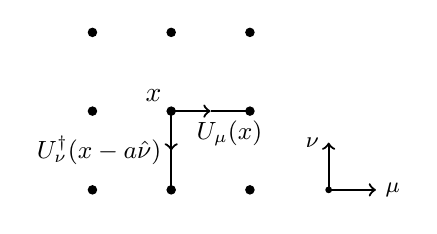
\begin{tikzpicture}
	\filldraw (0,0) circle (1.5pt);
	\filldraw (1,0) circle (1.5pt);
	\filldraw (2,0) circle (1.5pt);
	\filldraw (0,1) circle (1.5pt);
	\filldraw (1,1) circle (1.5pt);
	\filldraw (2,1) circle (1.5pt);
	\filldraw (0,2) circle (1.5pt);
	\filldraw (1,2) circle (1.5pt);
	\filldraw (2,2) circle (1.5pt);

	\draw [thick, ->] (1,1) -- (1.5,1);
	\draw [thick] (1.5,1) -- (2,1);
	\draw [thick, ->] (1,1) -- (1,0.5);
	\draw [thick] (1,0.5) -- (1,0);
	
	\filldraw (3,0) circle (1pt);
	\draw [thick, ->] (3,0) -- (3,0.6);
	\draw [thick, ->] (3,0) -- (3.6,0);
	\node[left] at (3,0.6) {\footnotesize $\nu$};
	\node[right] at (3.6,0) {\footnotesize $\mu$};

	\node[below right] at (1.2,1) {\small $U_\mu(x)$};
	\node[left] at (1,0.5) {\small $U^\dagger_\nu(x-a\hat{\nu})$};
	\node[above left] at (1,1) {$x$};
\end{tikzpicture}
\caption{Two link variables on the $\mu\nu$ plane. Reverse directions are represented by the inverse of the link variable.} \label{fig:LinkVar}
\end{figure}

The simplest path that can be created is the plaquette as shown in figure \ref{fig:Plaq}. Mathematically, this can be written as
\begin{align}
	P_{\mu\nu}=\frac{1}{3}\Re\Trace(U_\mu(x)U\nu(x+a\hat{\mu})U_\mu^\dagger(x+a\hat{\nu})U_\nu^\dagger(x)).
	\label{eq:Plaq}
\end{align}

\begin{figure}[h]
\centering
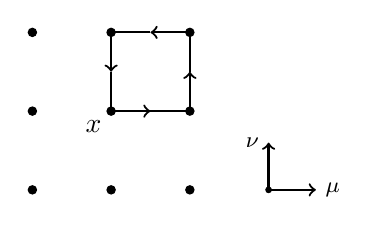
\begin{tikzpicture}
	\filldraw (0,0) circle (1.5pt);
	\filldraw (1,0) circle (1.5pt);
	\filldraw (2,0) circle (1.5pt);
	\filldraw (0,1) circle (1.5pt);
	\filldraw (1,1) circle (1.5pt);
	\filldraw (2,1) circle (1.5pt);
	\filldraw (0,2) circle (1.5pt);
	\filldraw (1,2) circle (1.5pt);
	\filldraw (2,2) circle (1.5pt);
	
	\draw [thick, ->] (1,1) -- (1.5,1);	\draw [thick] (1.5,1) -- (2,1);
	\draw [thick, ->] (2,1) -- (2,1.5);	\draw [thick] (2,1.5) -- (2,2);
	\draw [thick, ->] (2,2) -- (1.5,2);	\draw [thick] (1.5,2) -- (1,2);
	\draw [thick, ->] (1,2) -- (1,1.5);	\draw [thick] (1,1.5) -- (1,1);
	
	\filldraw (3,0) circle (1pt);
	\draw [thick, ->] (3,0) -- (3,0.6);
	\draw [thick, ->] (3,0) -- (3.6,0);
	\node[left] at (3,0.6) {\footnotesize $\nu$};
	\node[right] at (3.6,0) {\footnotesize $\mu$};

	\node[below left] at (1,1) {$x$};
\end{tikzpicture}
\caption{The plaquette which is the simplest guage invariant object that can be created from the link variables.} \label{fig:Plaq}
\end{figure}
With this, the Wilson gauge action is
\begin{align}
	S=\beta\sum_x\sum_{\mu>\nu}[1-P_{\mu\nu}(x)]
	\label{eq:WilsonAction}
\end{align}
where $\beta=6/g^2$ is the lattice coupling. The Wilson action is base on Wilson loops where the plaquette is an example of the simplest Wilson loop. It is the normalized ordered product of links in a path. It's used in equation \ref{eq:WilsonAction} and will be used in the improved action derived shortly. For small $a$, if we expand the plaquette at some $x_0$ as a polynomial in $a$, due to $A_\mu$ being slowly varying because $a$ is small, we find
\begin{align}
	P_{\mu\nu}=1-\frac{a^4}{6}\Trace(gF_\mu\nu(x_0))^2+\mathcal{O}(a^6)
\end{align}
where $F_{\mu\nu}=\partial_\mu A_\nu-\partial_\nu A_\mu+ig[A_\mu,A_\nu]$ is the field strength tensor. Taking the continuum limit $a\to0$, what remains is the continuum action up to second-order shown in equation \ref{eq:ContAction}.
\begin{align}
	S=\int\dd[4]{x}\frac{1}{2}\sum_{\mu,\nu}\Trace F_{\mu\nu}^2(x)
	\label{eq:ContAction}
\end{align}
These higher-order terms complicate the action as such:
\begin{align}
	S=\int\dd[4]{x}\sum_{\mu,\nu}\left[\frac{1}{2}\Trace F_{\mu\nu}^2(x)+\frac{a^2}{24}\Trace F_{\mu\nu}(D_\mu^2+D_\nu^2)F_{\mu\nu}+\ldots\right]
\end{align}
The terms $D_\mu$ and $D_\nu$ are gauge covariant derivatives for their respective directions.

To cancel out the higher-order term, we can introduce the rectangle operator. Similar to the plaquette in equation \ref{eq:Plaq}, it is the normalized real trace of the path in figure \ref{fig:Rect}.
\begin{figure}[h]
\centering
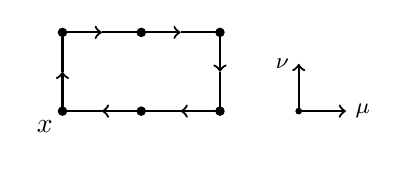
\begin{tikzpicture}
	\filldraw (0,0) circle (1.5pt);
	\filldraw (1,0) circle (1.5pt);
	\filldraw (2,0) circle (1.5pt);
	\filldraw (0,1) circle (1.5pt);
	\filldraw (1,1) circle (1.5pt);
	\filldraw (2,1) circle (1.5pt);
	
	\draw [thick, ->] (0,0) -- (0,0.5); \draw [thick] (0,0.5) -- (0,1);
	\draw [thick, ->] (0,1) -- (0.5,1); \draw [thick] (0.5,1) -- (1,1);
	\draw [thick, ->] (1,1) -- (1.5,1); \draw [thick] (1.5,1) -- (2,1);	
	\draw [thick, ->] (2,1) -- (2,0.5); \draw [thick] (2,0.5) -- (2,0);
	\draw [thick, ->] (2,0) -- (1.5,0); \draw [thick] (1.5,0) -- (1,0);
	\draw [thick, ->] (1,0) -- (0.5,0); \draw [thick] (0.5,0) -- (0,0);

	\filldraw (3,0) circle (1pt);
	\draw [thick, ->] (3,0) -- (3,0.6);
	\draw [thick, ->] (3,0) -- (3.6,0);
	\node[left] at (3,0.6) {\footnotesize $\nu$};
	\node[right] at (3.6,0) {\footnotesize $\mu$};

	\node[below left] at (0,0) {$x$};
\end{tikzpicture}
\caption{The rectangle operator at point $x$.} \label{fig:Rect}
\end{figure}
The rectangle operator has as an expansion
\begin{align}
	R_{\mu\nu}=1-\frac{4a^4}{6}\Trace(gF_{\mu\nu})^2-\frac{4a^6}{72}\Trace(gF_{\mu\nu}(4D_\mu^2+D_\nu^2)gF_{\mu\nu})+\mathcal{O}(a^8).
\end{align}
With the different coefficients for the $a^4$ and $a^6$ terms, an improved action can be calculated which is accurate up to third-order:
\begin{align}
	S_{imp}=-\beta\sum_x\sum_{\mu>\nu}\left[\frac{5}{3}P_{\mu\nu}-\frac{1}{12}(R_{\mu\nu}+R_{\nu\mu})\right].
	\label{eq:ImpAct}
\end{align}
One last modification to the above action is necessary for an accurate quantum action, that is an action that can accurately describe this system. This is the tadpole improvement, a renormalization $\mu_0$ that accounts for the extra terms in the action. Then equation \ref{eq:ImpAct} becomes
\begin{align}
	S_{imp}=-\beta\sum_x\sum_{\mu>\nu}\left[\frac{5}{3\mu_0^4}P_{\mu\nu}-\frac{1}{12\mu_0^6}(R_{\mu\nu}+R_{\nu\mu})\right]
	\label{eq:ImpActTPI}
\end{align}
where the $\mu_0$'s cancel the tadpole contributions. The $\mu_0$'s depend only on the lattice spacing and can be found numerically; for example, for a lattice spacing of $a=0.4$ fm, then $\mu_0\approx3/4$. In this case, the contribution by the rectangle operators is increased by about a factor of 2 compared to the action without the tadpole improvement. With the action in equation \ref{eq:ImpActTPI}, Monte Carlo steps can be used to run this model.

\subsection{Monte Carlo Application}
Again, the steps of Monte Carlo in this context is analogous to before. There are added complications that must be sorted out and, in doing so, increase the computing time appreciably. As stated before, the lattice is four-dimensional to account for three spacial dimensions and one temporal dimension. Furthermore, the calculations for the model exist at the links of which each lattice site has four.

We begin by looking at an $N$x$N$x$N$x$N$ lattice with coordinates $(x,\ y,\ z,\ t)$ at the site $x$ and the link in the $\hat{x}$ direction\footnote{In the code, the variable $n\in\{0,1,2,3\}$ is used to determine the specific link. This follows more easily with the sum in the action that is over $\mu>\nu$, thus $n_x=0\Leftrightarrow\hat{x}$, $n_y=1\Leftrightarrow\hat{y}$, etc.}. There are six plaquettes and twelve rectangle operators that affect the link $U_x(x)$ but for now we will focus only on the plaquettes. Figure \ref{fig:XPlane} shows these plaquettes. The plaquettes are equivalent for each plane that $U_x(x)$ is found on and the $yz$, $yt$ and $zt$ planes are not included (even though they are part of the sum in equation \ref{eq:ImpActTPI}) because they do not contain plaquettes of $U_x(x)$ and therefore do not contribute to the action for this link. So for any link, three of the planes will not contribute. It is important to note that each plane has a contribution of $U_\mu(x)$ and of $U_\mu^\dagger(x)$ for some $\mu$-direction.

\begin{figure}[h]
\centering
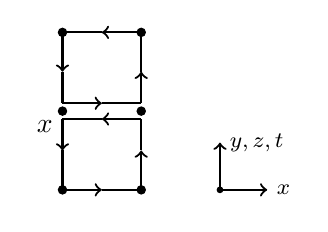
\begin{tikzpicture}
	\filldraw (0,0) circle (1.5pt);
	\filldraw (1,0) circle (1.5pt);
	\filldraw (0,1) circle (1.5pt);
	\filldraw (1,1) circle (1.5pt);
	\filldraw (0,2) circle (1.5pt);
	\filldraw (1,2) circle (1.5pt);
	
	\draw [thick, ->] (0,1.1) -- (0.5,1.1); \draw [thick] (0.5,1.1) -- (1,1.1);
	\draw [thick, ->] (1,1.1) -- (1,1.5); \draw [thick] (1,1.5) -- (1,2);
	\draw [thick, ->] (1,2) -- (0.5,2); \draw [thick] (0.5,2) -- (0,2);
	\draw [thick, ->] (0,2) -- (0,1.5); \draw [thick] (0,1.5) -- (0,1.1);
	
	\draw [thick, ->] (0,0.9) -- (0,0.5); \draw [thick] (0,0.5) -- (0,0);
	\draw [thick, ->] (0,0) -- (0.5,0); \draw [thick] (0.5,0) -- (1,0);
	\draw [thick, ->] (1,0) -- (1,0.5); \draw [thick] (1,0.5) -- (1,0.9);
	\draw [thick, ->] (1,0.9) -- (0.5,0.9); \draw [thick] (0.5,0.9) -- (0,0.9);

	\filldraw (2,0) circle (1pt);
	\draw [thick, ->] (2,0) -- (2,0.6);
	\draw [thick, ->] (2,0) -- (2.6,0);
	\node[right] at (2,0.6) {\footnotesize $y,z,t$};
	\node[right] at (2.6,0) {\footnotesize $x$};

	\node[below left] at (0,1) {$x$};
\end{tikzpicture}
\caption{Two plaquettes that effect the link $U_x(x)$ with one being the inverse path or $U_x^\dagger(x)$. Since the lattice is four dimensional, the three planes of $x$ are analogous for calculation of $U_x(x)$.} \label{fig:XPlane}
\end{figure}

The picture for $U_t(x)$ is slightly different. Because $n_t>n_i$ for all $i\in\{x,y,z\}$, the plaquette at site $x$ contains the inverse link of $U_t(x)$. Thus the plaquette at site $x-a\hat{\mu}$ must be used as the plaquette containing $U_t(x)$ as shown in figure \ref{fig:TPlane}. For links in the $t$-direction, this is always true while for links in the $x$-direction, this is never true. The application of this can be seen in the code in figure \ref{fig:ComputePlaqStaples} which will be discribed shortly.

\begin{figure}[h]
\centering
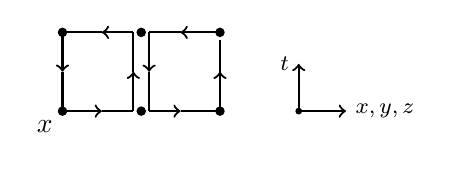
\begin{tikzpicture}
	\filldraw (0,0) circle (1.5pt);
	\filldraw (1,0) circle (1.5pt);
	\filldraw (2,0) circle (1.5pt);
	\filldraw (0,1) circle (1.5pt);
	\filldraw (1,1) circle (1.5pt);
	\filldraw (2,1) circle (1.5pt);
	
	\draw [thick, ->] (0,0) -- (0.5,0); \draw [thick] (0.5,0) -- (0.9,0);
	\draw [thick, ->] (0.9,0) -- (0.9,0.5); \draw [thick] (0.9,0.5) -- (0.9,1);
	\draw [thick, ->] (0.9,1) -- (0.5,1); \draw [thick] (0.5,1) -- (0,1);
	\draw [thick, ->] (0,1) -- (0,0.5); \draw [thick] (0,0.5) -- (0,0);
	
	\draw [thick, ->] (1.1,1) -- (1.1,0.5); \draw [thick] (1.1,0.5) -- (1.1,0);
	\draw [thick, ->] (1.1,0) -- (1.5,0); \draw [thick] (1.5,0) -- (2,0);
	\draw [thick, ->] (2,0) -- (2,0.5); \draw [thick] (2,0.5) -- (2,0.9);
	\draw [thick, ->] (2,1) -- (1.5,1); \draw [thick] (1.5,1) -- (1.1,1);

	\filldraw (3,0) circle (1pt);
	\draw [thick, ->] (3,0) -- (3,0.6);
	\draw [thick, ->] (3,0) -- (3.6,0);
	\node[left] at (3,0.6) {\footnotesize $t$};
	\node[right] at (3.6,0) {\footnotesize $x,y,z$};

	\node[below left] at (0,0) {$x$};
\end{tikzpicture}
\caption{Two plaquettes that effect the link $U_t(x)$. This picture holds for the planes where $\mu>\nu$.} \label{fig:TPlane}
\end{figure}

The rectangle operators are analogous but there is one important difference. Since these operators are $a\cross2a$ and not $a\cross a$ as are the plaquettes, there are more contributions to the operator. This can be seen in figure \ref{fig:RectOp}. As with the plaquette, the paths in this figure are for the $x$-direction but these paths will not be so for the $t$-direction. Rather, there is a rotation as before and for the same reason. Also, from equation \ref{eq:ImpActTPI}, there are terms $R_{\mu\nu}$ and $R_{\nu\mu}$. Thus there are six rectangle operators, double the number of plaquettes. For $U_x(x)$, there are only two staples for $R_{\nu\mu}$ and four for $R_{\mu\nu}$ and vis versa for $U_t(x)$. The staple being defined as the path operator without the path link in question. To sum up, if $n_\mu>n_\nu$, then $R_{\mu\nu}$ will be a sum of four staples and $R_{\nu\mu}$ will be the sum of two.
\begin{figure}[h]
\centering
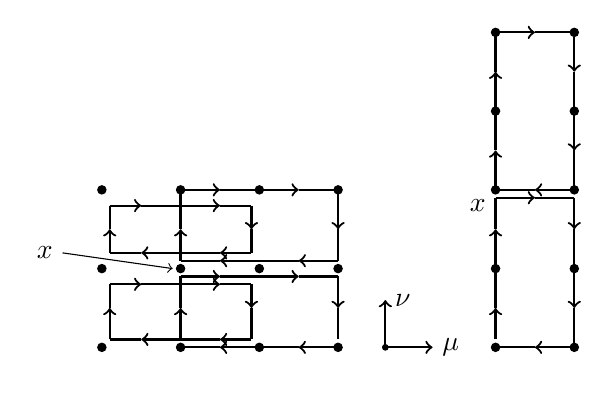
\begin{tikzpicture}
	\filldraw (0,0) circle (1.5pt);
	\filldraw (1,0) circle (1.5pt);
	\filldraw (2,0) circle (1.5pt);
	\filldraw (3,0) circle (1.5pt);
	\filldraw (0,1) circle (1.5pt);
	\filldraw (1,1) circle (1.5pt);
	\filldraw (2,1) circle (1.5pt);
	\filldraw (3,1) circle (1.5pt);
	\filldraw (0,2) circle (1.5pt);
	\filldraw (1,2) circle (1.5pt);
	\filldraw (2,2) circle (1.5pt);
	\filldraw (3,2) circle (1.5pt);

	\filldraw (5,0) circle (1.5pt);
	\filldraw (6,0) circle (1.5pt);
	\filldraw (5,1) circle (1.5pt);
	\filldraw (6,1) circle (1.5pt);
	\filldraw (5,2) circle (1.5pt);
	\filldraw (6,2) circle (1.5pt);
	\filldraw (5,3) circle (1.5pt);
	\filldraw (6,3) circle (1.5pt);
	\filldraw (5,4) circle (1.5pt);
	\filldraw (6,4) circle (1.5pt);
	
	\draw [thick, ->] (1,1.1) -- (1,1.5); \draw [thick] (1,1.5) -- (1,2);
	\draw [thick, ->] (1,2) -- (1.5,2); \draw [thick] (1.5,2) -- (2,2);
	\draw [thick, ->] (2,2) -- (2.5,2); \draw [thick] (2.5,2) -- (3,2);	
	\draw [thick, ->] (3,2) -- (3,1.5); \draw [thick] (3,1.5) -- (3,1.1);
	\draw [thick, ->] (3,1.1) -- (2.5,1.1); \draw [thick] (2.5,1.1) -- (2,1.1);
	\draw [thick, ->] (2,1.1) -- (1.5,1.1); \draw [thick] (1.5,1.1) -- (1,1.1);
	
	\draw [thick, ->] (1,0.1) -- (1,0.5); \draw [thick] (1,0.5) -- (1,0.9);
	\draw [thick, ->] (1,0.9) -- (1.5,0.9); \draw [thick] (1.5,0.9) -- (2,0.9);
	\draw [thick, ->] (2,0.9) -- (2.5,0.9); \draw [thick] (2.5,0.9) -- (3,0.9);	
	\draw [thick, ->] (3,0.9) -- (3,0.5); \draw [thick] (3,0.5) -- (3,0.1);
	\draw [thick, ->] (3,0) -- (2.5,0); \draw [thick] (2.5,0) -- (2,0);
	\draw [thick, ->] (2,0) -- (1.5,0); \draw [thick] (1.5,0) -- (1,0);
	
	\draw [thick, ->] (0.1,1.2) -- (0.1,1.5); \draw [thick] (0.1,1.5) -- (0.1,1.8);
	\draw [thick, ->] (0.1,1.8) -- (0.5,1.8); \draw [thick] (0.5,1.8) -- (0.9,1.8);
	\draw [thick, ->] (0.9,1.8) -- (1.5,1.8); \draw [thick] (1.5,1.8) -- (1.9,1.8);	
	\draw [thick, ->] (1.9,1.8) -- (1.9,1.5); \draw [thick] (1.9,1.5) -- (1.9,1.2);
	\draw [thick, ->] (1.9,1.2) -- (1.5,1.2); \draw [thick] (1.5,1.2) -- (0.9,1.2);
	\draw [thick, ->] (0.9,1.2) -- (0.5,1.2); \draw [thick] (0.5,1.2) -- (0.1,1.2);	

	\draw [thick, ->] (0.1,0.1) -- (0.1,0.5); \draw [thick] (0.1,0.5) -- (0.1,0.8);
	\draw [thick, ->] (0.1,0.8) -- (0.5,0.8); \draw [thick] (0.5,0.8) -- (0.9,0.8);
	\draw [thick, ->] (0.9,0.8) -- (1.5,0.8); \draw [thick] (1.5,0.8) -- (1.9,0.8);	
	\draw [thick, ->] (1.9,0.8) -- (1.9,0.5); \draw [thick] (1.9,0.5) -- (1.9,0.1);
	\draw [thick, ->] (1.9,0.1) -- (1.5,0.1); \draw [thick] (1.5,0.1) -- (0.9,0.1);
	\draw [thick, ->] (0.9,0.1) -- (0.5,0.1); \draw [thick] (0.5,0.1) -- (0.1,0.1);		
	
	\draw [thick, ->] (5,0.1) -- (5,0.5); \draw [thick] (5,0.5) -- (5,1);
	\draw [thick, ->] (5,1) -- (5,1.5); \draw [thick] (5,1.5) -- (5,1.9);
	\draw [thick, ->] (5,1.9) -- (5.5,1.9); \draw [thick] (5.5,1.9) -- (6,1.9);
	\draw [thick, ->] (6,1.9) -- (6,1.5); \draw [thick] (6,1.5) -- (6,1);
	\draw [thick, ->] (6,1) -- (6,0.5); \draw [thick] (6,0.5) -- (6,0);
	\draw [thick, ->] (6,0) -- (5.5,0); \draw [thick] (5.5,0) -- (5,0);
	
	\draw [thick, ->] (5,2) -- (5,2.5); \draw [thick] (5,2.5) -- (5,3);
	\draw [thick, ->] (5,3) -- (5,3.5); \draw [thick] (5,3.5) -- (5,4);
	\draw [thick, ->] (5,4) -- (5.5,4); \draw [thick] (5.5,4) -- (6,4);
	\draw [thick, ->] (6,4) -- (6,3.5); \draw [thick] (6,3.5) -- (6,3);
	\draw [thick, ->] (6,3) -- (6,2.5); \draw [thick] (6,2.5) -- (6,2);
	\draw [thick, ->] (6,2) -- (5.5,2); \draw [thick] (5.5,2) -- (5,2);
	
	\filldraw (3.6,0) circle (1pt);
	\draw[thick, ->] (3.6,0) -- (3.6,0.6);
	\draw[thick, ->] (3.6,0) -- (4.2,0);
	\node[right] at (3.6,0.6) {$\nu$};
	\node[right] at (4.2,0) {$\mu$};
	
	\node[below left] at (5,2) {$x$};
	\draw[->] (-0.5,1.2) -- (0.9,1);
	\node[left] at (-0.5,1.2) {$x$};
\end{tikzpicture}
\caption{The possible configurations of the rectangle operator. Depending on the direction, the rectangles may be rotated as with the plaquettes. For $U_t(x)$, the rectangles are rotated 90$^\circ$ relative to $U_x(x)$.} \label{fig:RectOp}
\end{figure}

In the code in \ref{fig:ComputePlaqStaples}, the function \texttt{nPlaq} calculates the staple and conjugate staple for the link at lattice site $(x,\ y,\ z,\ t,\ n)$ where $n$ specifies the link. The values \texttt{staples} and \texttt{stapleC} are the sums of the staples and conjugate staples, respectively. They are used to calculate $\Delta S$ (along with the rectangle staples for the improved action).
\begin{figure}[h]
\begin{lstlisting}
def nPlaq(x, y, z, t, n):
    a = [0] * 4
    a[n] = 1
    staples = 0
    stapleC = 0

    for i in range(3 - n):
        staples += mm(L[m(x+a[0])][m(y+a[1])][m(z+a[2])][t][n+i+1],
                        ct(L[x][m(y+a[-i])][m(z+a[1-i])][m(t+a[2-i])][n]),
                        ct(L[x][y][z][t][n+i+1]))
        stapleC += mm(ct(L[x][m(y-a[-i])][m(z-a[1-i])][m(t-a[2-i])][n+i+1]),
                        L[x][m(y-a[-i])][m(z-a[1-i])][m(t-a[2-i])][n],
                        L[m(x+a[0])][m(y+a[1]-a[-i])][m(z+a[2]-a[1-i])][t-a[2-i]][n+i+1])
    for i in range(n):
        staples += mm(ct(L[m(x-a[i+n])][m(y-a[i+n-1]+a[1])][m(z-a[i+n-2]+a[2])][m(t+a[3])][i]),
                        ct(L[m(x-a[i+n])][m(y-a[i+n-1])][m(z-a[i+n-2])][t][n]),
                        L[m(x-a[i+n])][m(y-a[i+n-1])][m(z-a[i+n-2])][t][i])
        stapleC += mm(L[x][y][z][t][i],
                        L[m(x+a[i+n])][m(y+a[i+n-1])][m(z+a[i+n-2])][t][n],
                        ct(L[x][m(y+a[1])][m(z+a[2])][m(t+a[3])][i]))
    return staples, stapleC
\end{lstlisting}
\caption{Python code for calculating the regular and conjugate transpose staples for $U_\mu(x)$, a link in direction $n_\mu$. The two for loops are to account for the change in the calculation of the staples for each link direction.}
\label{fig:ComputePlaqStaples}
\end{figure}

In the previous model, a small random change $\epsilon$ was added to a time slice for a path $x$ and the resulting change in the action was calculated. The same is done again except the path links are $SU(3)$ matrices, not numbers, so a `small' random $SU(3)$ matrix is added to the path link, that is a matrix close to the identity. Thus we take $U\to MU$ if $U$ is a path link and $M\in SU(3)$ is close to the identity. The small change in $U$ is given by the product $MU$ which is also an $SU(3)$ matrix since $SU(3)$ is a group and thus is closed under this operation. This resulting change is used to calculate the change in the action, $\Delta S$.

Let $\mathcal{S}_{\mu\nu}(C)$ represent the staple(s)\footnote{Here I say ``staple(s)" because there can be more than one staple coming from the $\mu\nu$ plane like with the rectangle operator (where there can be two). It is implied these are being summed first in the equation which is more useful as a template for visualizing $\Delta S$ than a rigorous formula.} for $U_\mu(x)$ in the $\mu\nu$ plane for path $C$ and $\mathcal{S}^*_{\mu\nu}(C)$ be the staple(s) for $U_\mu^\dagger(x)$. Then the change in the unimproved action from equation \ref{eq:WilsonAction} for site $x$ is
\begin{align}
	\Delta S(x)=\frac{\beta}{3}\Re\Trace\left[(I-M)U_\mu(x)\sum_{\nu\neq\mu}\mathcal{S}_{\mu\nu}(P_{\mu\nu})+U^\dagger_\mu(x)(I-M^\dagger)\sum_{\nu\neq\mu}\mathcal{S}^*_{\mu\nu}(P_{\mu\nu})\right]
	\label{eq:MCNormAction}
\end{align}
and the improved action is
\begin{align}
\begin{split}
	\Delta S_{imp}(x)=\frac{\beta}{3}\Re\Trace\left[(I-M)U_\mu(x)\left(c_1\sum_{\nu\neq\mu}\mathcal{S}_{\mu\nu}(P_{\mu\nu})-c_2\sum_{\nu\neq\mu}[\mathcal{S}_{\mu\nu}(R_{\mu\nu})+\mathcal{S}_{\mu\nu}(R_{\nu\mu})]\right)\right.\\
	\left.+U^\dagger_\mu(x)(I-M^\dagger)\left(c_1\sum_{\nu\neq\mu}\mathcal{S}^*_{\mu\nu}(P_{\mu\nu})-c^2\sum_{\nu\neq\mu}[\mathcal{S}^*_{\mu\nu}(R_{\mu\nu})+\mathcal{S}^*_{\mu\nu}(R_{\nu\mu})\right)\right]
\end{split}
	\label{eq:MCImpAction}
\end{align}
where $M$ is a random $SU(3)$ matrix close to the identity, $c_1=5/3\mu_0^4$ and $c_2=1/12\mu_0^6$. With this in mind, one sweep of the lattice can be completed with the following steps:
\begin{enumerate}
\item Choose a site $x$ and a link $n$.
\item Choose a random $SU(3)$ matrix $M$ such that $U_\mu(x)\to MU_\mu(x)$.
\item Calculate the change in action $\Delta S$ with equation \ref{eq:MCImpAction}.
\item If $\Delta S<0$, then keep the change $MU_\mu(x)$.
\item Otherwise assign it a probability $\exp(-\Delta S)$ of changing.
\item Repeat steps 1-5 for every site on the path.
\end{enumerate}
These steps are very similar to those from before, the main changes coming in the equation for the action which is much more costly in this model; the lattice is higher dimensional and the Monte Carlo steps require more computations and are computed on matrices. In figure \ref{fig:LQCDSweep}, equation \ref{eq:MCImpAction} is implemented under \texttt{dS} where the matrices \text{staples} and \text{stapleC} are calculated as shown in figure \ref{fig:ComputePlaqStaples} and \texttt{rects} and \texttt{rectC} are calculated in a similar but longer function \texttt{nRect}. The $SU(3)$ matrices used as the small Monte Carlo variable are generated beforehand and stored in \texttt{SU3list} along with their inverses.
\begin{figure}[h]
\begin{lstlisting}
def dS(staples, stapleC, rects, rectC, x, y, z, t, n):
    M = SU3list[np.random.randint(0, 2 * numMatrices)]
    U = L[x][y][z][t][n]
    deltaS = (beta / 3) * np.real(np.trace(np.dot(U - mm(M, U), c1 * staples - c2 * rects) + \
                                        np.dot(ct(U) - ct(mm(M, U)), c1 * stapleC - c2 * rectC)))             
    return deltaS, M

def sweep():
    for p in product(range(N), range(N), range(N), range(N), range(4)):
        x, y, z, t, n = p
        staples, stapleC = nPlaq(x, y, z, t, n)
        rects, rectC = nRect(x,y,z,t,n)
        for _ in range(N_ma):
            deltaS, M = dS(staples, stapleC, rects, rectC, x, y, z, t, n)
            if deltaS < 0 or np.random.random() < np.exp(-deltaS):
                L[x][y][z][t][n] = np.dot(M, L[x][y][z][t][n])
\end{lstlisting}
\caption{The code that evolves the lattice. The array \texttt{L} is the lattice with $N^4*4$ sites given $N$ as the side length of the lattice and an $SU(3)$ matrix at each site with the total length of \texttt{L} being $36*N^4$. The function \texttt{sweep} completes a sweep of the lattice and \texttt{dS} calculates the change in the action. At each site $(x,\ y,\ z,\ t,\ n)$, the Metropolis algorithm is done \texttt{N\_ma} times so as to let the link variable reach an equilibrium with its neighbors before moving on to the next link.}
\label{fig:LQCDSweep}
\end{figure}

\subsection{Measurements}
With the derivation of the path integral in mind, we precede with the gluonic path integral similarly with $N=8$ as a lattice size\footnote{Even though this lattice size is much smaller than the previous, this simulation requires hours, compared to minutes, to complete 25 measurements with 50 sweeps between measurements. All code was run in Python 3.x on an Intel i7 processor on Windows 10.}. We can measure the effect of the Wilson loop operator on the vacuum state and, with the choice of Wilson loop, the measurement will change. First, the lattice is thermalized, as defined earlier, by completing 100 sweeps and then measurements are taken every $N_{cor}=50$ sweeps. The trace of the Wilson loops for each path link are summed and averaged. In figure \ref{fig:LQCDConv}, the convergence of the Wilson loops are shown. After 100 sweeps, the lattice has reach equilibrium and 50 sweeps is sufficiently long enough to prevent correlation in the measurements.

\begin{figure}[h]
	\centering
	\includegraphics[scale=0.60]{LQCD_Convergence.png}
	\caption{A visualization of the convergence rates of the Monte Carlo measurements. The first 100 sweeps, which are plotted, are used for reaching the equilibrium of the lattice and so measurements are not completed during these sweeps.}
	\label{fig:LQCDConv}
\end{figure}

The Monte Carlo averages of $a\cross a$, $a\cross2a$ and $a\cross3a$ Wilson loops are calculated as shown in the code in figure \ref{fig:LQCDMCCode}. In general, measurement of an arbitrary Wilson loop $W$ requires only a change in the product of the link variables.

The averages are also calculated for both the unimproved and improved actions:
\begin{align}
	S(x)=\frac{\beta}{\mu_0^4}\sum_{\mu>\nu}P_{\mu\nu}(x)\qquad\ S_{imp}(x)=-\beta\sum_{\mu>\nu}\left[\frac{5}{3\mu_0^4}P_{\mu\nu}-\frac{1}{12\mu_0^6}(R_{\mu\nu}+R_{\nu\mu})\right].
	\label{eq:ActAgain}
\end{align}
This allows us to visual the difference in the second- and third-order accuracy of the discretized action, i.e. the contribution of the rectangle operators. For the unimproved and improved actions, the averages, denoted by $\mathcal{W}$ and $\mathcal{W}_{imp}$, respectively, are
\begin{align}
\begin{split}
	\mathcal{W}(a\cross a)=0.497\pm0.003\qquad\quad&\mathcal{W}_{imp}(a\cross a)=0.546\pm0.003,\\
	\mathcal{W}(a\cross2a)=0.260\pm0.004\qquad\quad&\mathcal{W}_{imp}(a\cross2a)=0.290\pm0.004,\\
	\mathcal{W}(a\cross3a)=0.137\pm0.004\qquad\quad&\mathcal{W}_{imp}(a\cross3a)=0.156\pm0.003.
\end{split}
\end{align}
These are the unweighted means for the respective Wilson loops as shown in figure \ref{fig:LQCDMCCode}. These results suggest that the larger the area of the Wilson loop, the smaller $\mathcal{W}$ will be.
\begin{figure}[h!]
\begin{lstlisting}
def measure(loopLength):
    LAvg = 0
    for p in product(range(N), range(N), range(N), range(N)):
        x, y, z, t = p
        link = measureLink(x, y, z, t, loopLength)
        LAvg += np.real(np.trace( 
        mm(L[x][y][z][t][0], L[m(x+1)][y][z][t][1], link[0], ct(L[x][y][z][t][1])) + 
        mm(L[x][y][z][t][0], L[m(x+1)][y][z][t][2], link[1], ct(L[x][y][z][t][2])) + 
        mm(L[x][y][z][t][0], L[m(x+1)][y][z][t][3], link[2], ct(L[x][y][z][t][3])) + 
        mm(L[x][y][z][t][1], L[x][m(y+1)][z][t][2], link[3], ct(L[x][y][z][t][2])) + 
        mm(L[x][y][z][t][1], L[x][m(y+1)][z][t][3], link[4], ct(L[x][y][z][t][3])) + 
        mm(L[x][y][z][t][2], L[x][y][m(z+1)][t][3], link[5], ct(L[x][y][z][t][3]))))
    return LAvg / N**4 / 18
\end{lstlisting}
	\caption{Python code that measures an $a\cross ca$ Wilson loop for $c\in\{1,2,3\}$. The array \texttt{link} determines specific links in the loop based on \texttt{loopLength}. The returned value is the normalized average.}
	\label{fig:LQCDMCCode}
\end{figure}

\begin{figure}[h]
	\centering
	\includegraphics[scale=0.60]{LQCD_MC_Measurements.png}
	\caption{Monte Carlo measurements for $a\cross a$, $a\cross2a$ and $a\cross3a$ Wilson loops. The triangles represent the improved action from equation \ref{eq:ImpActTPI} while the squares represent the unimproved action from equation \ref{eq:WilsonAction}. Between each measurement, $N_{cor}=50$ sweeps were omitted along with 100 sweeps after the lattice was initialized for it to reach equilibrium.}
	\label{fig:LQCDPlot}
\end{figure}

With the system modeled based on the assumptions of the system, the measurements are relatively trivial in both computational time and in the complexity of the code. Further measurements can be made on this lattice or more realistic properties can be assumed for the lattice, although the latter may increase the computing time significantly due to its added complexity. Nevertheless, as with the previous models, the potential for added measurements exists.
\end{document}